\documentclass[11pt]{article}
\usepackage[margin=0.85in]{geometry}
\usepackage{graphicx}
\usepackage{booktabs}
\usepackage{longtable}
\usepackage{array}
\usepackage{hyperref}
\usepackage{float}
\usepackage{microtype}
\hypersetup{colorlinks=true, linkcolor=black, urlcolor=blue, citecolor=black}
\setlength{\parskip}{0.55em}
\setlength{\parindent}{0pt}
\newcolumntype{L}[1]{>{\raggedright\arraybackslash}p{#1}}

\title{Santiment Data Anomalies as Conditional Market-State Features:\\A Production-Audited Event Study on Binance-Tradable Crypto Assets}
\author{Santiment Research}
\date{June 1, 2026}

\begin{document}
\maketitle

\begin{abstract}
This paper evaluates four Santiment data anomalies as conditional market-state features: Social Dev Score, ETH Whale Dump, Price/Network Activity Divergence, and Project in Trends. The study combines production-audited definitions, production event rows, and Binance hourly USDT prices for mapped tradable assets. Events are compared with same-asset, same-quarter control timestamps over 1h, 4h, 24h, and 72h horizons. The strongest evidence is concentrated in Price/Network Activity Divergence, which shows positive event-minus-control signed returns and materially higher realized volatility. Project in Trends behaves more like an attention and risk-state marker: post-event realized volatility rises while 24h signed returns are negative in this sample. ETH Whale Dump remains an ETH-specific event-risk label, and Social Dev Score has limited statistical evidence after the Binance and sparse-asset filters. These findings should be interpreted as conditional event-state evidence. They are not a transaction-cost-aware trading strategy, out-of-sample validation, or standalone proof of alpha.
\end{abstract}

\section{Executive Overview}
The final evaluated sample contains 1,211 unique events across 34 mapped Binance-tradable assets. The source window is 2023-01-01 through 2026-05-28, with effective coverage differing by data anomaly because production history and price coverage differ. The strongest 24h directional result is Price/Network Activity Divergence: event-minus-control forward return is 2.14 percentage points with FDR q=0.018. The strongest volatility result is also Price/Network Activity Divergence: 24h realized volatility is 2.17 percentage points above controls with FDR q=0.002. Project in Trends shows higher 24h realized volatility but negative 24h signed return. ETH Whale Dump and Social Dev Score do not provide strong 24h directional evidence in this run.

The practical read is conservative. These data anomalies are useful as context features for alerts, dashboards, risk-state interpretation, and research workflows. They are not yet transaction-cost-aware portfolio rules. The current Binance-tradable asset map should also be treated as a study filter, not as proof that all events were tradable with sufficient liquidity at the historical event time.

\section{What Santiment Data Anomalies Are}
Santiment data anomalies are production-generated event labels. They indicate that a metric, behavior, or social/on-chain state has moved into an unusual condition according to detector-specific logic. They are not all designed to be directional return predictors. Some are better interpreted as attention shocks, volatility warnings, event-risk markers, or regime/context features.

In this paper, an anomaly event is treated as \texttt{asset x timestamp x data anomaly}. The paper asks what tends to happen after these events relative to comparable non-event timestamps for the same asset.

This distinction matters for client interpretation. A data anomaly can be useful even when its signed-return effect is weak, if it reliably identifies a higher-volatility state, an attention shock, or a period where additional due diligence is warranted.

\section{Data Anomaly Coverage and Production Definitions}
The asset universe is restricted to mapped Binance spot USDT markets. Events outside that universe are excluded. The study uses UTC timestamps and Binance hourly closes. The production audit is treated as the source of truth for data anomaly semantics; where detector logic or upstream tables are not fully observable, the limitation is carried into the interpretation.

\begin{table}[H]
\centering
\caption{Evaluated events after Binance price-coverage filtering.}
\begin{tabular}{lrrrr}
\toprule
Data Anomaly & Events & Assets & First Event & Last Event \\
\midrule
ETH Whale Dump & 87 & 1 & 2023-09-11 & 2026-05-25 \\
Price/Network Activity Divergence & 255 & 22 & 2023-01-03 & 2026-05-08 \\
Project in Trends & 803 & 18 & 2025-01-01 & 2026-05-27 \\
Social Dev Score & 66 & 11 & 2023-01-01 & 2026-05-06 \\
\bottomrule
\end{tabular}
\end{table}

\textbf{Social Dev Score} is a composite developer/social activity-state anomaly. It combines ranked GitHub activity and social-volume inputs, then requires both an elevated composite score and an unusually high rolling z-score. \textbf{ETH Whale Dump} is an ETH-only filtered large-holder flow event, based on large net ETH outflow behavior over a roughly 30-day transaction window. \textbf{Price/Network Activity Divergence} flags cases where smoothed price appreciation is unusually high relative to smoothed daily active address growth. \textbf{Project in Trends} detects mapped projects appearing in top social trending words from Reddit, crypto Twitter, and Telegram sources with cooldown behavior.

Two coverage caveats are important. First, the Binance-tradable universe is a current mapped universe, not a complete historical exchange-availability and liquidity screen. Second, Project in Trends is highly concentrated: the top three evaluated assets are bitcoin, ethereum, solana (65.4\% of events). This concentration supports asset-weighted inference and limits broad cross-sectional claims.

\section{Evaluation Framework}
Each event is compared with 10 control timestamps sampled from the same asset, preferably in the same calendar quarter, while excluding timestamps close to same-asset anomaly events. Outcomes are signed forward return, absolute return, and realized volatility over 1h, 4h, 24h, 72h windows. Multi-asset headline estimates are asset-weighted to reduce domination by high-frequency assets; ETH Whale Dump is event-weighted because it is ETH-only. Confidence intervals use bootstrap sampling and p-values are adjusted with Benjamini-Hochberg FDR across the headline tests.

This is an event study, not a market-model abnormal-return study. Controls are not explicitly matched on hour-of-week, liquidity, volatility regime, or broad crypto market factors. The design is therefore appropriate for conditional event-state evidence, but it does not isolate a pure risk-adjusted return premium. It is not a transaction-cost-aware portfolio backtest, does not model order execution, and does not infer deployable capacity.

\section{Key Empirical Findings}
Table abbreviations are EWD for ETH Whale Dump, PNAD for Price/Network Activity Divergence, PIT for Project in Trends, and SDSC for Social Dev Score. FwdRet is signed forward return and RV is realized volatility. All differences are event minus control, in percentage points.

\begin{longtable}{lllrp{2.8cm}rrr}
\caption{Primary event-control effects. Differences are event minus control, in percentage points.}\\
\toprule
Data Anomaly & Horizon & Metric & Diff. & 95\% CI & FDR q & Events & Assets \\
\midrule
\endfirsthead
\toprule
Data Anomaly & Horizon & Metric & Diff. & 95\% CI & FDR q & Events & Assets \\
\midrule
\endhead
EWD & 4h & FwdRet & 0.074 & [-0.253, 0.434] & 0.8014 & 87 & 1 \\
EWD & 24h & FwdRet & 0.040 & [-0.611, 0.751] & 0.9489 & 87 & 1 \\
EWD & 72h & FwdRet & -0.663 & [-1.798, 0.449] & 0.4296 & 86 & 1 \\
EWD & 4h & RV & 0.311 & [0.066, 0.588] & 0.0530 & 87 & 1 \\
EWD & 24h & RV & 0.276 & [-0.102, 0.676] & 0.3149 & 87 & 1 \\
EWD & 72h & RV & -0.113 & [-0.629, 0.470] & 0.8014 & 86 & 1 \\
PNAD & 4h & FwdRet & 0.535 & [0.054, 1.021] & 0.1059 & 255 & 22 \\
PNAD & 24h & FwdRet & 2.137 & [0.987, 3.443] & 0.0178 & 255 & 22 \\
PNAD & 72h & FwdRet & 4.642 & [2.285, 7.459] & 0.0153 & 255 & 22 \\
PNAD & 4h & RV & 0.933 & [0.553, 1.314] & 0.0020 & 255 & 22 \\
PNAD & 24h & RV & 2.165 & [1.413, 3.008] & 0.0016 & 255 & 22 \\
PNAD & 72h & RV & 3.636 & [2.339, 5.119] & 0.0016 & 255 & 22 \\
PIT & 4h & FwdRet & -0.349 & [-0.849, 0.099] & 0.3149 & 803 & 18 \\
PIT & 24h & FwdRet & -1.476 & [-2.449, -0.520] & 0.0318 & 803 & 18 \\
PIT & 72h & FwdRet & -2.725 & [-5.359, -0.360] & 0.1059 & 799 & 18 \\
PIT & 4h & RV & 0.620 & [0.315, 0.957] & 0.0144 & 803 & 18 \\
PIT & 24h & RV & 1.587 & [0.696, 2.577] & 0.0186 & 803 & 18 \\
PIT & 72h & RV & 2.427 & [1.209, 3.713] & 0.0153 & 799 & 18 \\
SDSC & 4h & FwdRet & -0.720 & [-1.670, 0.120] & 0.3111 & 66 & 11 \\
SDSC & 24h & FwdRet & 0.492 & [-1.266, 3.218] & 0.8082 & 66 & 11 \\
SDSC & 72h & FwdRet & 0.652 & [-4.546, 6.914] & 0.9081 & 66 & 11 \\
SDSC & 4h & RV & 0.186 & [-0.346, 0.839] & 0.7370 & 66 & 11 \\
SDSC & 24h & RV & 0.574 & [-0.621, 2.083] & 0.6174 & 66 & 11 \\
SDSC & 72h & RV & 0.722 & [-0.785, 2.678] & 0.6174 & 66 & 11 \\
\bottomrule
\end{longtable}

\begin{figure}[H]
\centering
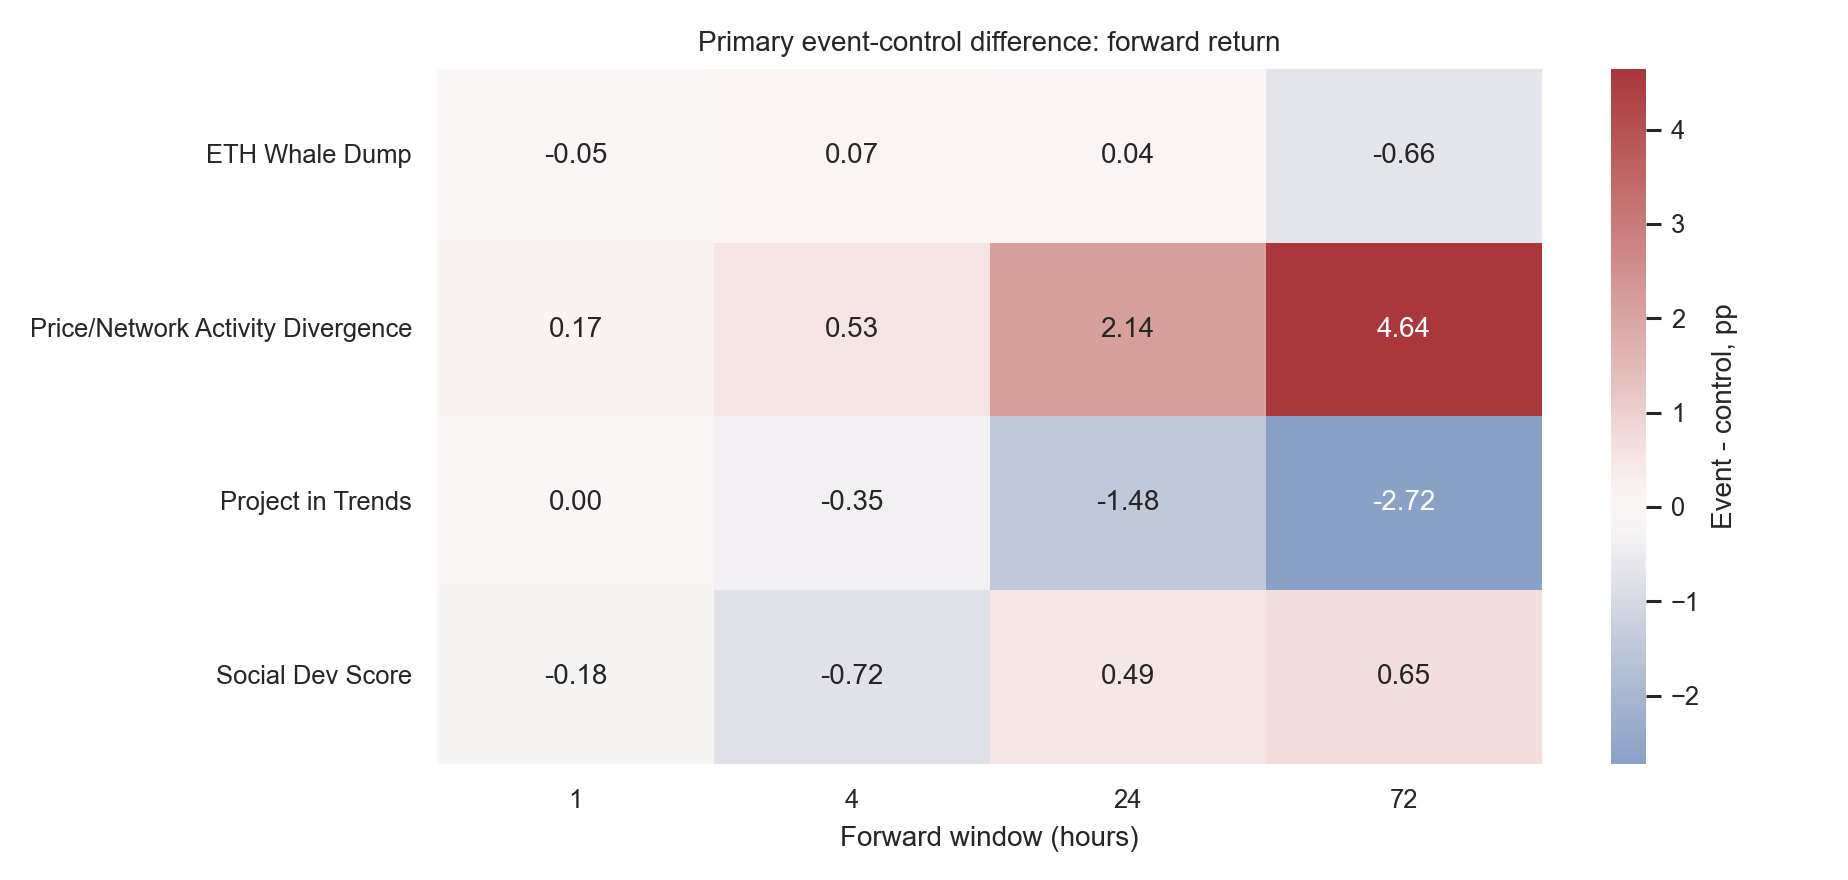
\includegraphics[width=0.9\linewidth]{figures/forward_return_heatmap.png}
\caption{Primary signed forward-return effects.}
\end{figure}

\begin{figure}[H]
\centering
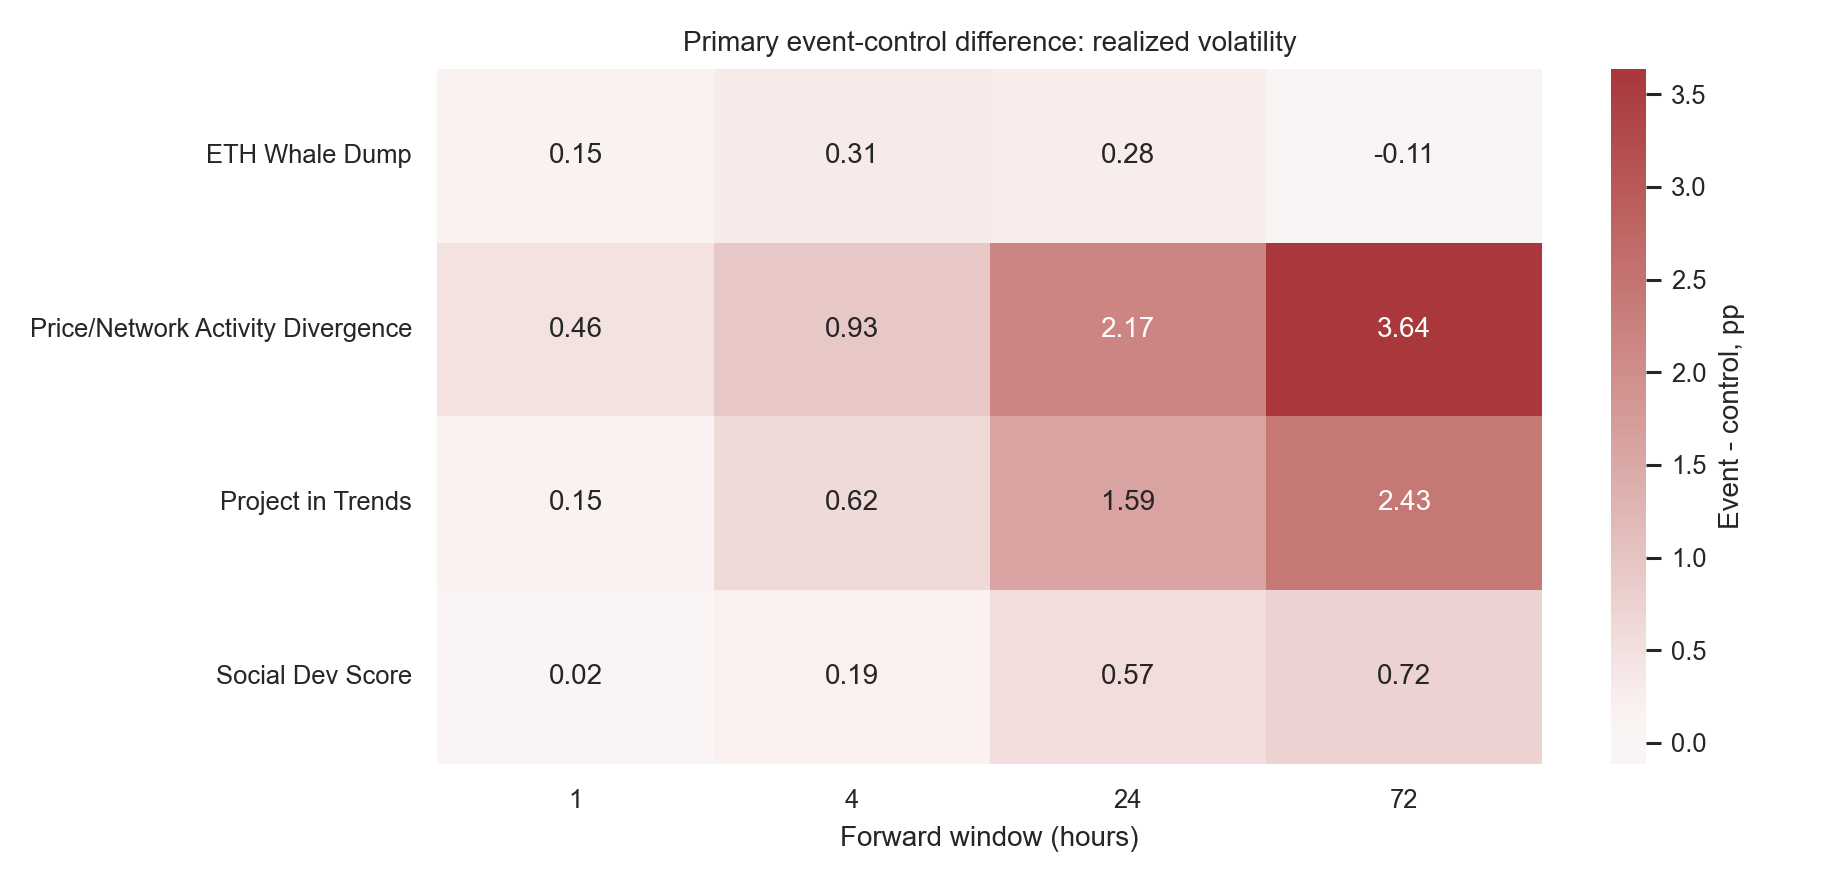
\includegraphics[width=0.9\linewidth]{figures/realized_volatility_heatmap.png}
\caption{Primary realized-volatility effects.}
\end{figure}

The main empirical pattern is that data anomalies are more reliable as state features than as uniform directional predictors. Price/Network Activity Divergence is the exception worth deeper follow-up: both its 24h return effect and 24h realized-volatility effect are positive and FDR-significant in this sample. Its largest five evaluated asset buckets are lido-dao, bonk1, bitcoin-cash, dogecoin, 0x (33.7\% of events), so the result is not driven by a single asset. Project in Trends is better read as attention/risk-state evidence: 24h return is -1.48 percentage points while 24h realized volatility is 1.59 percentage points above controls. ETH Whale Dump and Social Dev Score have weak 24h signed-return evidence: 0.04 and 0.49 percentage points respectively.

\section{Anomaly-by-Anomaly Interpretation}
\textbf{Social Dev Score.} Production meaning: composite developer/social activity score shock. Empirical evidence: limited after the Binance and sparse-asset filters. Return effect: weak and noisy. Volatility/risk effect: positive point estimates but wide intervals. Asset concentration is material: the largest five evaluated assets are litecoin, ethereum-classic, dogecoin, ethereum, bitcoin (71.2\% of events). Recommended use: dashboard context or research feature, not a standalone entry rule.

\textbf{ETH Whale Dump.} Production meaning: ETH-only filtered large-holder flow event. Empirical evidence: better interpreted as event-risk context than directional return evidence. Return effect: near zero at 24h in this run. Volatility/risk effect: mildly positive at short horizons but not robust at 24h. Recommended use: ETH risk marker and alert context.

\textbf{Price/Network Activity Divergence.} Production meaning: price growth unusually high relative to network activity growth. Empirical evidence: strongest of the four data anomalies. Return effect: positive at 24h and 72h in the tested sample. Volatility/risk effect: consistently elevated. Recommended use: candidate for deeper portfolio backtest and regime-aware validation.

\textbf{Project in Trends.} Production meaning: project appears in top social trending-word sets. Empirical evidence: strong attention/risk-state interpretation. Return effect: negative at 24h in this sample. Volatility/risk effect: elevated and more stable than signed return. Recommended use: attention shock feature, alert context, and volatility warning.

\begin{table}[H]
\centering
\small
\caption{Reviewer evidence grades. Grades summarize this study only; they are not product labels.}
\begin{tabular}{L{0.22\linewidth}L{0.16\linewidth}L{0.26\linewidth}L{0.20\linewidth}}
\toprule
Data Anomaly & Evidence Grade & Best Current Use & Main Caveat \\
\midrule
Price/Network Activity Divergence & B & Candidate for deeper portfolio validation; volatility-state feature & No costs, liquidity screen, or out-of-sample test \\
Project in Trends & B for attention/risk; C for direction & Attention shock and volatility warning & Concentrated in large assets and social-source mapping \\
ETH Whale Dump & C & ETH-specific event-risk context & Single-asset sample, weak 24h direction \\
Social Dev Score & D+ & Research/dashboard context & Sparse and concentrated sample \\
\bottomrule
\end{tabular}
\end{table}

\section{How Clients Should Use These Data Anomalies}
Clients should use these anomalies as conditional context rather than direct trading instructions. The best product fit is to combine them with asset liquidity, market regime, user watchlists, and independent confirmation metrics. Price/Network Activity Divergence can be prioritized for strategy research. Project in Trends and Social Dev Score fit dashboard and alert workflows. ETH Whale Dump fits ETH-specific risk monitoring.

Good uses include: ranking assets for further review, explaining unusual market states, triggering watchlist alerts, adding context to risk dashboards, and selecting candidates for formal strategy research.

The recommended product wording is conditional: "this data anomaly has historically coincided with higher volatility" or "this event has historically marked an attention shock." Avoid wording that implies a direct buy/sell recommendation or guaranteed post-event price move.

\section{What These Data Anomalies Do Not Prove}
These results do not prove standalone alpha. They do not include transaction costs, slippage, exchange availability history, borrow constraints, portfolio construction, position sizing, live-trading delays, or liquidity capacity. They do not prove that users should buy or sell after an alert. They also do not prove that effects are stable across future regimes, non-Binance venues, illiquid assets, or different detector thresholds.

The results are conditional event-study evidence. A trading claim would require a separate portfolio-level study with costs, execution assumptions, out-of-sample validation, risk controls, and a pre-specified decision rule. Without those layers, the correct interpretation is "state information," not "deployable alpha."

\section{Conclusion}
The evidence supports treating Santiment data anomalies as conditional market-state features. The price-network divergence anomaly is the strongest candidate for directional follow-up. Project in Trends is most useful as an attention and volatility-state anomaly. ETH Whale Dump is an ETH-specific event-risk marker. Social Dev Score is inconclusive in this filtered sample.

Before any of these data anomalies are described as alpha, they should be validated in a cost-aware portfolio backtest.

\appendix
\section{Methodology Details}
The source window is 2023-01-01 00:00:00 UTC through 2026-05-28 00:00:00 UTC. The event sample is restricted to assets with mapped Binance spot USDT markets and sufficient per-asset event count for the relevant data anomaly. Events that cannot be matched to required forward price coverage are excluded from the evaluated event-window rows.

Controls are sampled from the same asset and, where available, the same calendar quarter as the event. Each event has 10 sampled controls per horizon. Control timestamps close to same-asset anomaly events are excluded using a horizon-dependent exclusion window. Outcomes are computed from Binance hourly close prices. Signed return is the percentage price change from event timestamp to horizon endpoint. Realized volatility is the square root of summed squared hourly log returns within the forward window. Absolute return is the absolute value of signed return. Headline estimates are event minus control.

For multi-asset data anomalies, the headline estimate is asset-weighted so high-frequency assets do not dominate. ETH Whale Dump is event-weighted because all evaluated rows are ETH. Confidence intervals are bootstrap intervals. Reported q-values use Benjamini-Hochberg FDR adjustment across the headline tests. The design does not estimate market-model abnormal returns, double-clustered standard errors, intraday seasonality controls, or liquidity-adjusted effects.

\section{Production Audit Notes}
\begin{itemize}
\item Social Dev Score combines ranked social-volume and developer-activity inputs into a composite score. The audited detector uses a 30-day rolling baseline, a z-score threshold of 3, and a score threshold above 70. The value field is the composite score, with component scores carried in metadata.
\item ETH Whale Dump is ETH-only and should not be generalized to other assets. The audited detector uses a large net ETH outflow condition, with a 1500 ETH scale threshold and a roughly 30-day transaction-window condition.
\item Price/Network Activity Divergence is based on daily price and daily active address divergence. The audited detector smooths price and active-address inputs over a 3-day window, compares the price-to-network-activity ratio against a roughly 30-day history, and requires both a modified z-score threshold of 4 and at least 3\% price growth.
\item Project in Trends depends on social-source coverage, top-word ranking, project-to-asset mapping, and cooldown behavior. The audited detector uses Reddit, crypto Twitter, and Telegram sources, a top-10 trending-word set, and a 12-hour cooldown. Current production configuration excludes Bitcoin and Ethereum projects, while historical evaluated rows include BTC and ETH; this history/configuration mismatch is carried as a caveat.
\end{itemize}

\section{Reproducibility Notes}
No new data were fetched for this restructured draft. It reuses the existing CSVs, tables, figures, and manifest from \texttt{binance\_anomaly\_paper\_20260528}. Source script: \texttt{run\_binance\_anomaly\_paper.py}. Restructuring script: \texttt{build\_restructured\_paper.py}. Manifest path: \texttt{manifest.json}. Price source: Binance spot USDT hourly close via \texttt{anomaly\_evaluation.fetching.BinanceDataFetcher}. Timezone: UTC for event timestamps. Random seed for the original event/control sampling: 20260528.

\section{Additional Tables and Figures}
\begin{figure}[H]
\centering
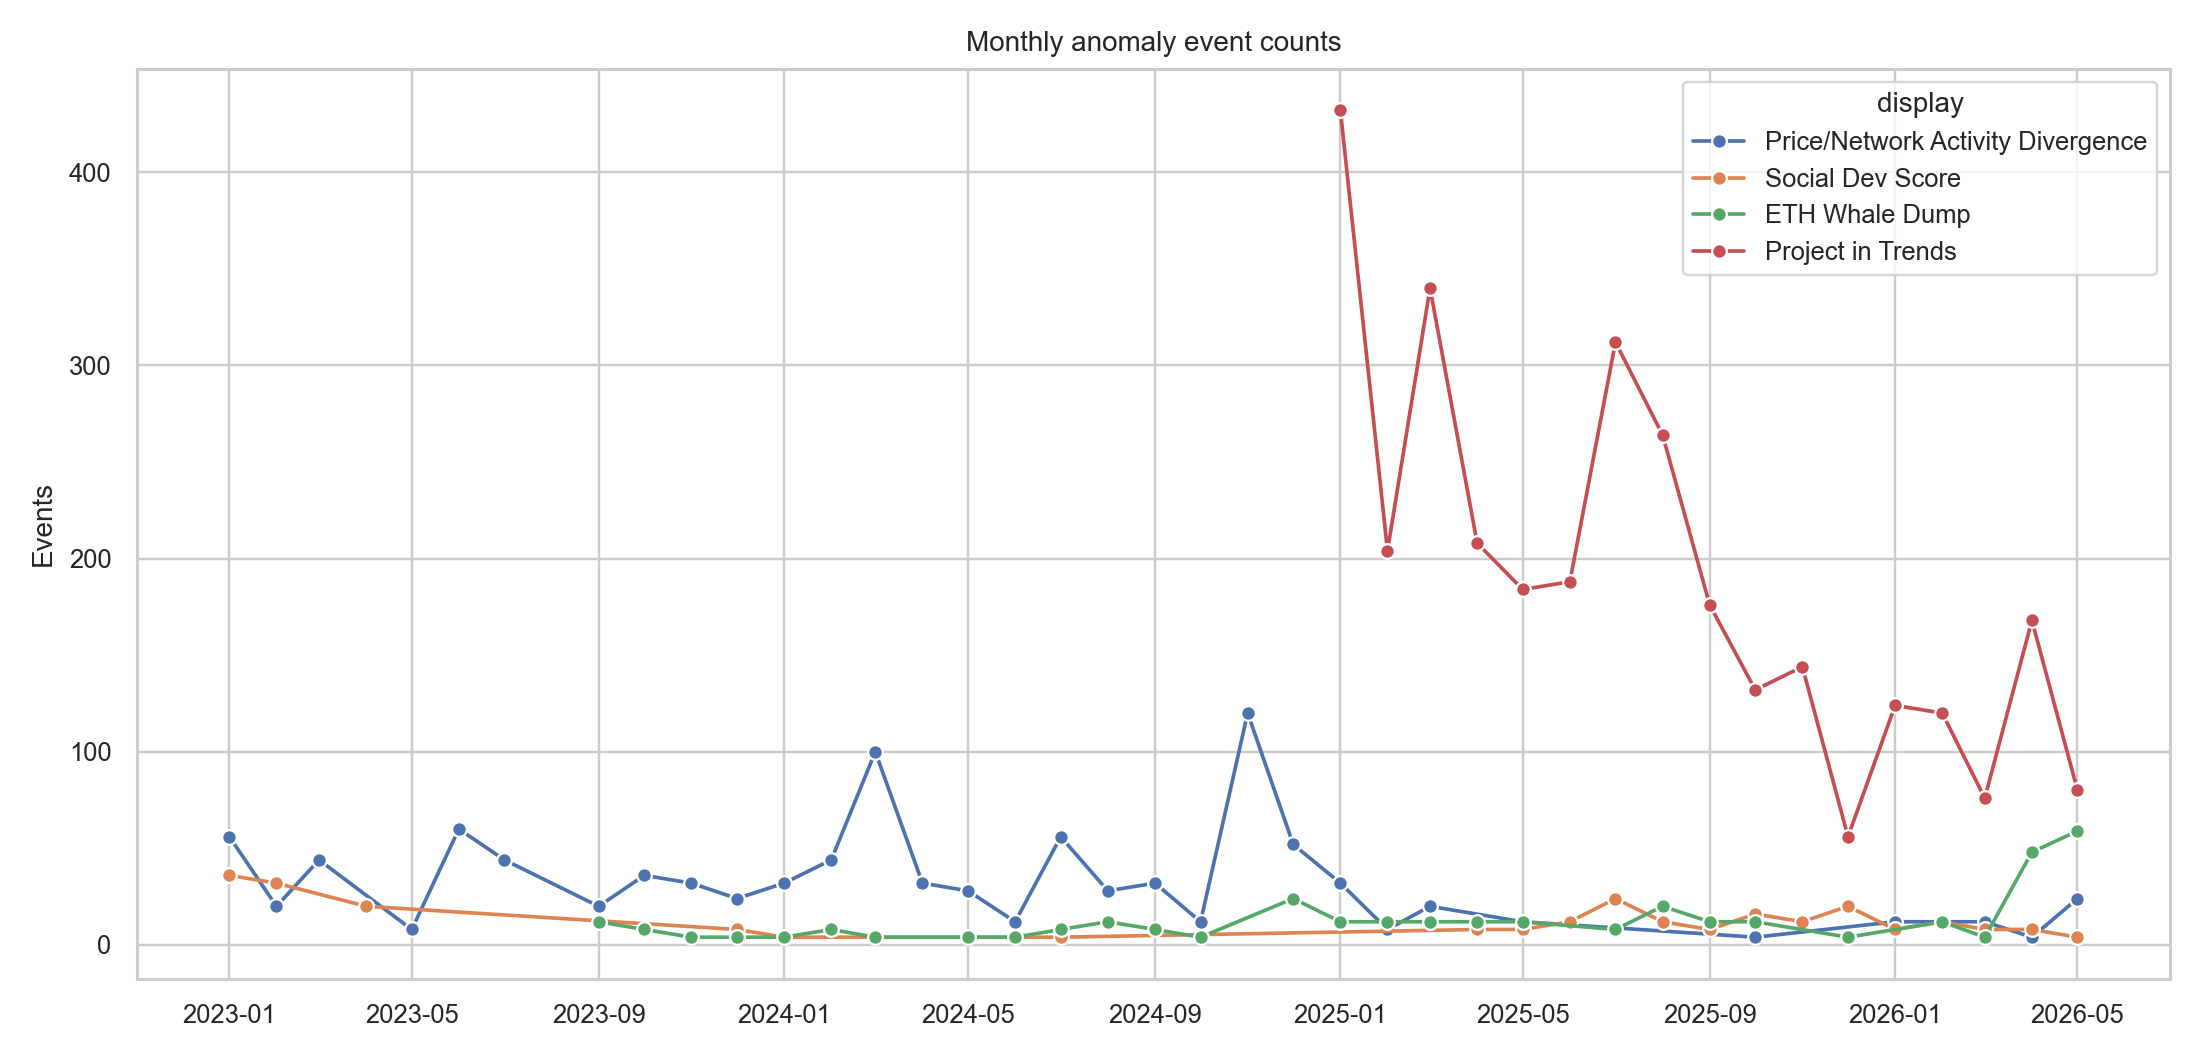
\includegraphics[width=0.9\linewidth]{figures/monthly_event_counts.png}
\caption{Monthly anomaly event counts.}
\end{figure}

\begin{figure}[H]
\centering
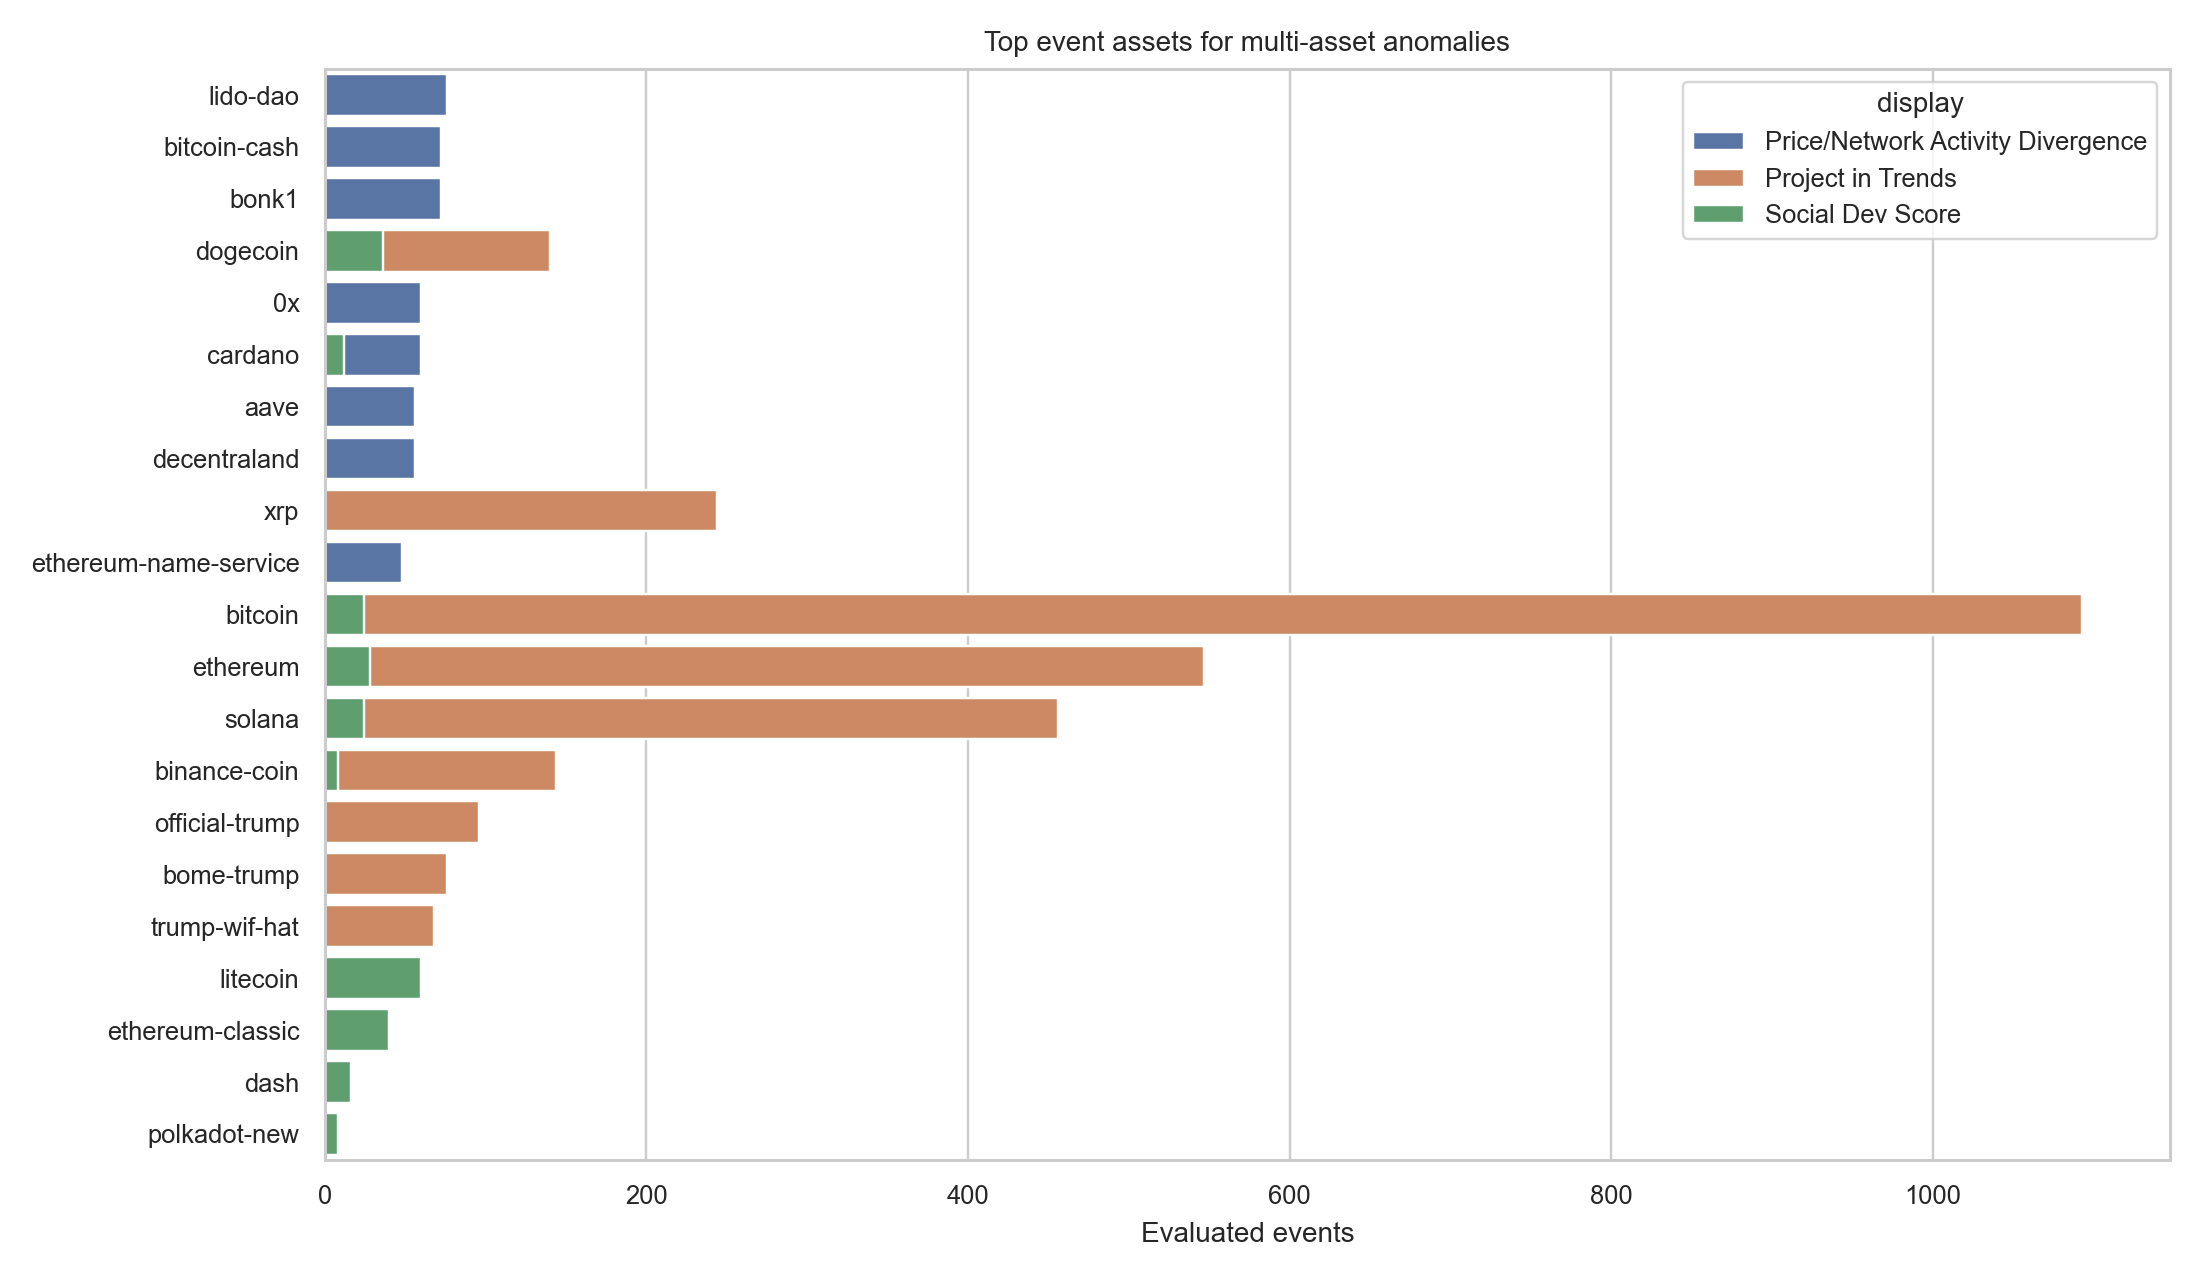
\includegraphics[width=0.9\linewidth]{figures/top_assets.png}
\caption{Top event assets for multi-asset anomalies.}
\end{figure}

\begin{figure}[H]
\centering
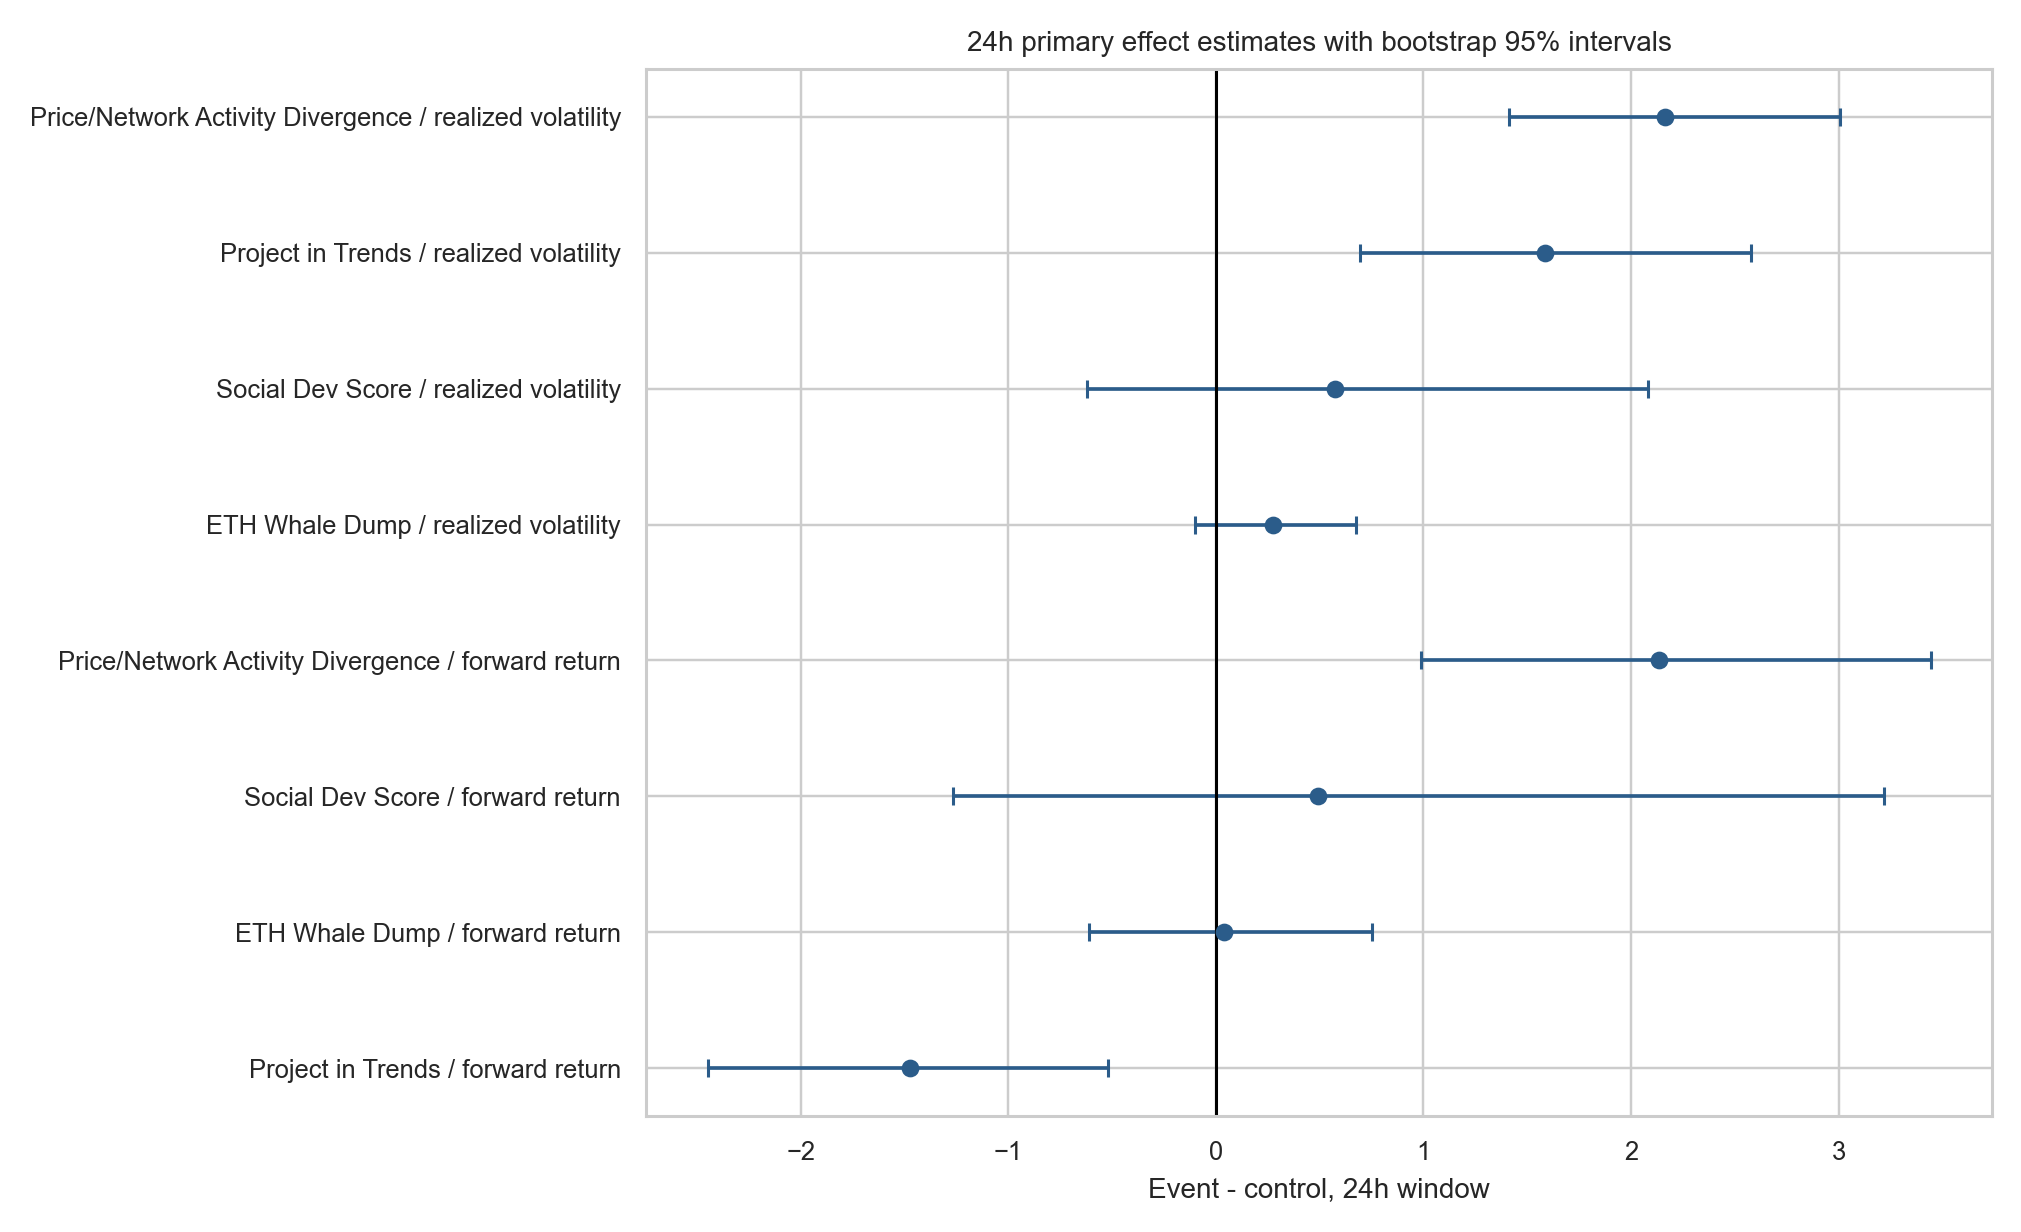
\includegraphics[width=0.9\linewidth]{figures/effect_forest_24h.png}
\caption{24h primary effect estimates with bootstrap 95\% intervals.}
\end{figure}

\begin{thebibliography}{99}
\bibitem{mackinlay1997} MacKinlay, A. C. (1997). Event Studies in Economics and Finance. \emph{Journal of Economic Literature}, 35(1), 13--39.
\bibitem{brownwarner1985} Brown, S. J., and Warner, J. B. (1985). Using Daily Stock Returns: The Case of Event Studies. \emph{Journal of Financial Economics}, 14(1), 3--31.
\bibitem{benjamini1995} Benjamini, Y., and Hochberg, Y. (1995). Controlling the False Discovery Rate. \emph{Journal of the Royal Statistical Society: Series B}, 57(1), 289--300.
\bibitem{harvey2016} Harvey, C. R., Liu, Y., and Zhu, H. (2016). ... and the Cross-Section of Expected Returns. \emph{Review of Financial Studies}, 29(1), 5--68.
\bibitem{bailey2014} Bailey, D. H., and Lopez de Prado, M. (2014). The Deflated Sharpe Ratio. \emph{Journal of Portfolio Management}, 40(5), 94--107.
\bibitem{barberodean2008} Barber, B. M., and Odean, T. (2008). All That Glitters. \emph{Review of Financial Studies}, 21(2), 785--818.
\bibitem{da2011} Da, Z., Engelberg, J., and Gao, P. (2011). In Search of Attention. \emph{Journal of Finance}, 66(5), 1461--1499.
\bibitem{makarovschoar2020} Makarov, I., and Schoar, A. (2020). Trading and Arbitrage in Cryptocurrency Markets. \emph{Journal of Financial Economics}, 135(2), 293--319.
\end{thebibliography}

\end{document}
